\documentclass[a4paper,12pt]{extarticle}
\usepackage{geometry}
\usepackage[T1]{fontenc}
\usepackage[utf8]{inputenc}
\usepackage[english,russian]{babel}
\usepackage{amsmath}
\usepackage{amsthm}
\usepackage{amssymb}
\usepackage{fancyhdr}
\usepackage{setspace}
\usepackage{graphicx}
\usepackage{colortbl}
\usepackage{tikz}
\usepackage{pgf}
\usepackage{subcaption}
\usepackage{listings}
\usepackage{indentfirst}
\usepackage[
backend=biber,
style=numeric,
maxbibnames=99
]{biblatex}
\addbibresource{refs.bib}
\usepackage[colorlinks,citecolor=blue,linkcolor=blue,bookmarks=false,hypertexnames=true, urlcolor=blue]{hyperref} 
\usepackage{indentfirst}
\usepackage{mathtools}
\usepackage{booktabs}
\usepackage[flushleft]{threeparttable}
\usepackage{tablefootnote}

\usepackage{chngcntr} % нумерация графиков и таблиц по секциям
\counterwithin{table}{section}
\counterwithin{figure}{section}

\graphicspath{{graphics/}}%путь к рисункам

\makeatletter
% \renewcommand{\@biblabel}[1]{#1.} % Заменяем библиографию с квадратных скобок на точку:
\makeatother

% \geometry{left=2.5cm}% левое поле
% \geometry{right=1.0cm}% правое поле
\geometry{left=1.75cm}
\geometry{right=1.75cm}

\geometry{top=2.0cm}% верхнее поле
\geometry{bottom=2.0cm}% нижнее поле
\setlength{\parindent}{1.25cm}
\renewcommand{\baselinestretch}{1.5} % междустрочный интервал


\newcommand{\bibref}[3]{\hyperlink{#1}{#2 (#3)}} % biblabel, authors, year
\addto\captionsrussian{\def\refname{Список литературы (или источников)}} 

\renewcommand{\theenumi}{\arabic{enumi}}% Меняем везде перечисления на цифра.цифра
\renewcommand{\labelenumi}{\arabic{enumi}}% Меняем везде перечисления на цифра.цифра
\renewcommand{\theenumii}{.\arabic{enumii}}% Меняем везде перечисления на цифра.цифра
\renewcommand{\labelenumii}{\arabic{enumi}.\arabic{enumii}.}% Меняем везде перечисления на цифра.цифра
\renewcommand{\theenumiii}{.\arabic{enumiii}}% Меняем везде перечисления на цифра.цифра
\renewcommand{\labelenumiii}{\arabic{enumi}.\arabic{enumii}.\arabic{enumiii}.}% Меняем везде перечисления на цифра.цифра

% Мои пакеты
\usepackage{tabularx}
\usepackage{booktabs}


\begin{document}
\begin{titlepage}
\newpage

{\setstretch{1.0}
\begin{center}
ПРАВИТЕЛЬСТВО РОССИЙСКОЙ ФЕДЕРАЦИИ\\
ФГАОУ ВО НАЦИОНАЛЬНЫЙ ИССЛЕДОВАТЕЛЬСКИЙ УНИВЕРСИТЕТ\\
«ВЫСШАЯ ШКОЛА ЭКОНОМИКИ»
\\
\bigskip
Факультет компьютерных наук\\
Образовательная программа «Прикладная математика и информатика»
\end{center}
}

\vspace{7em}

\begin{center}
{\bf ВЫПУСКНАЯ КВАЛИФИКАЦИОННАЯ РАБОТА}\\
%Выберите какой у вас проект
{\bf Исследовательский проект на тему:}\\
%{\bf Программный проект на тему:}\\
%{\bf Отчет о командном программном проекте на тему:}\\
{\bf Оптимизация размера сенсоров для физики элементарных частиц}\\
\end{center}

\vspace{2em}

{\bf Выполнил студент: \vspace{2mm}}

{\setstretch{1.1}
\begin{tabular}{l@{\hskip 1.5cm}l}
группы \#БПМИ203, 4 курса & Зиманов Алихан
\end{tabular}}

% Обычно у вас есть один научный руководитель, и это человек, с которым вы работаете над проектом. Иногда по формальным причинам у вас будет руководитель (штатный сотрудник Вышки) и соруководитель (тот, с кем вы работаете), — об этом вам сообщит учебный офис (в случае с ВКР) или ЦППРиП (в случае с курсовым проектом). Также, если кто-то дополнительно вам помогал, то его можно указать как консультанта. 

%ваш официальный научник (из ВШЭ)
\vspace{1em}
{\bf Принял руководитель ВКР: \vspace{2mm}}

{\setstretch{1.1}
\begin{tabular}{l}
Болдырев Алексей Сергеевич\\
Научный сотрудник\\
Факультет компьютерных наук НИУ ВШЭ 
\end{tabular}}

% со-руководитель (если есть)
%\vspace{1em}
%{\bf Соруководитель: \vspace{2mm}}%это ваш официальный научник

%{\setstretch{1.1}
%\begin{tabular}{l}
%Петрова Надежда Александровна\\
%Инженер-исследователь\\
%ОАО Компания "Нейросети и деревья" 
%\end{tabular}}

% консультант (если есть)
%\vspace{1em}
%{\bf Консультант: \vspace{2mm}}%это ваш официальный научник

%{\setstretch{1.1}
%\begin{tabular}{l}
%Иванова Надежда Александровна\\
%Инженер-исследователь\\
%ОАО Компания "Нейросети и деревья" 
%\end{tabular}}

\vspace{\fill}

\begin{center}
Москва 2024
\end{center}

\end{titlepage}% это титульный лист - выберите подходящий вам из имеющихся в проекте вариантов (kr - курсовая работа у 3 курса, vkr - выпускная квалификационная работа у 4 курса)
\newpage
\setcounter{page}{2}

{
	\hypersetup{linkcolor=black}
	\tableofcontents
}

\newpage

\newpage

\section*{Аннотация}   % this is how to use russian
В исследованиях фундаментальных частиц, точность и эффективность измерения метрик имеет первостепенное значение. Данное исследование представляет новый подход к оптимизации размеров датчиков в электромагнитных калориметрах (ЭМК) Большого адронного коллайдера (БАК) для точной реконструкции энергии и позиции фотонов. Используя методы глубинного обучения, особенно адаптированные из области компьютерного зрения, мы стремимся идентифицировать оптимальную конфигурацию матрицы датчиков, которая максимизирует точность реконструкции энергии и позиции, учитывая ограничения по стоимости. Введя архитектуру модели, способную адаптироваться к различным размерам датчиков, данное исследование рассматривает баланс между высоким разрешением измерений и экономической целесообразностью. Предварительные результаты показывают, что специально адаптированная модель глубокого обучения может значительно улучшить дизайн датчиков, предлагая многообещающий путь для будущих экспериментальных физических установок. Эта работа не только способствует текущему дискурсу по оптимизации датчиков, но и демонстрирует потенциал глубинного обучения в продвижении исследований в области физики частиц.

\addcontentsline{toc}{section}{Аннотация}

\section*{Ключевые слова}
Физика элементарных частиц, оптимизация размера сенсоров, глубинное обучение, компьютерное зрение, реконструкция энергии фотонов, БАК, электромагнитные калориметры

\section*{Abstract}   % this is how to use russian
В исследованиях фундаментальных частиц, точность и эффективность измерения метрик имеет первостепенное значение. Данное исследование представляет новый подход к оптимизации размеров датчиков в электромагнитных калориметрах (ЭМК) Большого адронного коллайдера (БАК) для точной реконструкции энергии и позиции фотонов. Используя методы глубинного обучения, особенно адаптированные из области компьютерного зрения, мы стремимся идентифицировать оптимальную конфигурацию матрицы датчиков, которая максимизирует точность реконструкции энергии и позиции, учитывая ограничения по стоимости. Введя архитектуру модели, способную адаптироваться к различным размерам датчиков, данное исследование рассматривает баланс между высоким разрешением измерений и экономической целесообразностью. Предварительные результаты показывают, что специально адаптированная модель глубокого обучения может значительно улучшить дизайн датчиков, предлагая многообещающий путь для будущих экспериментальных физических установок. Эта работа не только способствует текущему дискурсу по оптимизации датчиков, но и демонстрирует потенциал глубинного обучения в продвижении исследований в области физики частиц.

\addcontentsline{toc}{section}{Abstract}

\section*{Keywords}
Физика элементарных частиц, оптимизация размера сенсоров, глубинное обучение, компьютерное зрение, реконструкция энергии фотонов, БАК, электромагнитные калориметры

\pagebreak

\section{Введение}



\section{Обзор литературы}

Машинное обучение достаточно широко используется в задачах физики высоких энергий. Основными примерами таких задач являются задачи реконструкции свойств элементарных частиц, проходящих через датчики по типу электромагнитных калориметров в Большом адронном коллайдере. Так как структура данных, собираемых калориметром является матрицей, состоящей из вещественных чисел и имеет некоторые сходства с фотографиями (см. далее), то многие работы вполне естественно адаптируют модели из области компьютерного зрения для решения задач физики высоких энергий.

\subsection{Предшествующие работы}

Одна из работ~\cite{Belayneh_2020} из данной области исследует использование методов глубинного обучения для генерации и реконструкции при столкновении частиц в физике высоких энергий. Авторы этой статьи решают две задачи:

\begin{itemize}
    \item Восстановление энергии и идентификация элементарных частиц;
    \item Моделирование ливня элементарных частиц на калориметр.
\end{itemize}

Обе задачи решаются с помощью методов глубинного обучения. Для первой задачи в качестве подходящих архитектур были выбраны полносвязная нейронная сеть, трехмерная сверточная сеть и модель основанная на GoogLeNet. Для задачи моделирования авторы статьи используют архитектуру 3DGAN, основанную на трехмерных сверточных слоях.

Всего рассматриваются четыре типа частиц: электроны $e$, фотоны $\gamma$, заряженные пионы $\pi$ и нейтральные пионы $\pi^0$ с зарядами равномерно распределенными между $10$ и $510$ GeV. (смотрите на Fig. 15 photon variable energy regression).

В другой статье~\cite{Di_Bello_2021} предлагается использовать методы компьютерного зрения и глубинного обучения для улучшения реконструкции потока частиц (PFlow) в экспериментах по физике высоких энергий. Алгоритмы PFlow предназначены для идентификации и измерения энергии частиц, образующихся в результате столкновений, что является критически важным для понимания фундаментальных физических процессов.

Ключевые моменты статьи:
\begin{itemize}
    \item Задача: Различение нейтральных частиц (таких как фотоны и нейтральные пионы) от заряженных частиц (например, заряженных пионов) в данных калориметра, особенно когда их энергетические отложения перекрываются.
    Предлагаемое решение: Использование моделей компьютерного зрения и глубокого обучения для анализа изображений калориметра и прямого предсказания распределения нейтральной энергии.
    \item Изученные модели: \begin{itemize}
        \item Сверточные нейронные сети (CNN): Включая UNet с блоками ResNet, подходящие для обычных геометрий калориметров.
        \item Графовые нейронные сети (GNN): Предлагают гибкость для нерегулярных геометрий и превосходят CNN по энергетическому и пространственному разрешению.
        \item Глубокие множества (DS): Еще один подход для нерегулярных геометрий с хорошей производительностью.
    \end{itemize}
    \item Супер-разрешение: В статье также исследуется использование глубокого обучения для супер-разрешения, что позволяет восстанавливать изображения с более высокой детализацией, чем собственное разрешение детектора. Это может быть полезно для идентификации частиц и проектирования будущих детекторов.
    \item Результаты: Предложенные модели глубокого обучения значительно улучшают реконструкцию энергетических отложений нейтральных частиц по сравнению с традиционными параметрическими методами PFlow. Они достигают лучшего энергетического разрешения, пространственного разрешения и уменьшают смещение.
\end{itemize}

Дополнительные соображения:
В статье рассматривается упрощенный сценарий, включающий только заряженные и нейтральные пионы. Оценка производительности в более сложных событиях с несколькими типами частиц является критически важной.
Исследование других архитектур глубокого обучения и стратегий обучения может привести к дальнейшим улучшениям.
Важно исследовать вычислительные затраты и возможность реализации этих методов в реальных экспериментальных условиях.

В целом, эта статья представляет собой перспективный подход к реконструкции PFlow с использованием компьютерного зрения и глубокого обучения, предлагая потенциальные достижения в исследованиях по физике высоких энергий.

В данной статье~\cite{Akchurin_2021} исследуется потенциал глубинных нейронных сетей, в частности сверточных нейронных сетей (CNN) и графовых нейронных сетей (GNN), для реконструкции энергии частиц в высокогранулированных калориметрах. Авторы сравнивают эти методы с традиционными методами реконструкции энергии и обнаруживают, что CNN и GNN предлагают значительные преимущества, особенно в улучшении энергетического разрешения для адронных ливней.

Ключевые выводы:

\begin{itemize}
    \item CNN превосходят традиционные методы: CNN, обученная на смоделированных пионных ливнях, продемонстрировала существенное улучшение энергетического разрешения как для одиночных пионов, так и для струй по сравнению с традиционными методами, такими как простое суммирование энергии и коррекция fem (аналогично двухканальным калориметрам).
    \item CNN эффективны для различных типов частиц: CNN также показала хорошую производительность для реконструкции электронов и фотонов, даже несмотря на то, что она была обучена только на пионах.
    \item Понимание преимуществ CNN: Исследование предполагает, что CNN достигают превосходного разрешения, используя скрытые особенности пространственного распределения отложения энергии, которое коррелирует с физикой адронных ливней (например, множественность и угол рождения вторичных частиц).
    \item GNN и информация о времени: Включение информации о времени с помощью GNN еще больше улучшает энергетическое разрешение, особенно при точных измерениях времени ниже 100 пикосекунд.
    \item Потенциал для одноканальных калориметров: Способность CNN оценивать fem и fhad предполагает возможность достижения высокоточной реконструкции энергии с помощью одноканальных калориметров, устраняя необходимость в сложных многоканальных конструкциях.
\end{itemize}

В целом, это исследование подчеркивает перспективный потенциал методов глубокого обучения для продвижения технологии калориметров и достижения более точной реконструкции энергии в будущих экспериментах по физике высоких энергий.

В следующей статье~\cite{Wemmer_2023} исследуется применение графовых нейронных сетей (GNN) для реконструкции фотонов в электромагнитном калориметре (ECL) эксперимента Belle II. Цель состоит в улучшении энергетического разрешения и снижении фонового шума, особенно при высоких уровнях светимости.

Основные проблемы:

\begin{itemize}
    \item Высокий уровень фонового излучения пучка: Повышенная светимость приводит к большему фоновому шуму, что влияет на энергетическое разрешение.
    \item Перекрывающиеся фотоны: Важно различать энергетические отложения от нескольких фотонов.
    \item Сложная геометрия детектора: ECL имеет неоднородную структуру с кристаллами разных размеров и форм.
\end{itemize}

Предложенное решение:

\begin{itemize}
    \item Нечеткая кластеризация с использованием GNN: Этот подход назначает кристаллы разным классам (например, фотоны, фон) с различной степенью принадлежности.
    \item Архитектура GNN: Сеть использует блоки GravNet для изучения пространственных и характеристических представлений, а затем передает сообщения между связанными узлами.
    \item Входные данные: Используются свойства кристаллов (положение, масса), измерения (энергия, время, дискриминация формы импульса) и усредненные характеристики области интереса.
\end{itemize}

Результаты:

\begin{itemize}
    \item Значительное улучшение энергетического разрешения: Более чем на 30\% улучшение для фотонов низкой энергии и высокого фонового излучения пучка по сравнению с базовым алгоритмом.
    \item Сокращение хвостов в распределении энергии: GNN эффективно уменьшает фоновый шум, что приводит к более точной реконструкции энергии.
    \item Улучшенная производительность для перекрывающихся фотонов: Сеть успешно разделяет энергетические отложения от нескольких фотонов, особенно для асимметричных пар энергий.
    \item Многообещающая устойчивость к изменяющимся фонам пучка: GNN демонстрирует способность к обобщению на разные уровни фонового излучения.
\end{itemize}

Это исследование демонстрирует потенциал GNN для реконструкции калориметров в экспериментах по физике высоких энергий. Значительные улучшения в энергетическом разрешении и подавлении фона имеют прямые последствия для физических возможностей Belle II, особенно для анализов, связанных с фотонами и недостающей энергией.

\subsection{Используемые методы}

ResNet, Vision Transformer, Image augmentations

\section{Метод}

\subsection{Постановка задачи}

\subsection{Модели}

\subsection{Идеи обучения}

\section{Эксперименты}

\subsection{Данные}

\subsection{Метрики}

\subsection{Процесс обучения и замеров}

\subsection{Аугментации}

\section{Результаты}

\begin{table}[ht]
	\footnotesize
	\centering
	\begin{tabular}{llrrrrrrr}
		\toprule
		{} & {} & \multicolumn{6}{c}{\textsf{Размер матрицы}} \\
		\cmidrule(lr){3-8}
		\textsf{Модель} & \textsf{Метрика} & $\mathsf{10 \times 10}$ &  $\mathsf{15 \times 15}$ &  $\mathsf{20 \times 20}$ &  $\mathsf{25 \times 25}$ &  $\mathsf{30 \times 30}$ &  $\mathsf{40 \times 40}$ \\
		\midrule
        \textsf{SumModel} & $\mathcal{L}_{\mathsf{total}}$ & $\mathsf{0.1549}$ & $\mathsf{0.1555}$ & $\mathsf{0.1563}$ & $\mathsf{0.1575}$ & $\mathsf{0.1560}$ & $\mathsf{0.1561}$ \\
        {} & $\mathcal{L}_{\mathsf{eng}}$ & $\mathsf{0.0213}$ & $\mathsf{0.0221}$ & $\mathsf{0.0226}$ & $\mathsf{0.0229}$ & $\mathsf{0.0220}$ & $\mathsf{0.0222}$ \\
        {} & $\mathcal{L}_{\mathsf{pos}}$ & $\mathsf{0.2887}$ & $\mathsf{0.2891}$ & $\mathsf{0.2901}$ & $\mathsf{0.2924}$ & $\mathsf{0.2901}$ & $\mathsf{0.2901}$ \\
        \midrule
        \textsf{LinearModel} & $\mathcal{L}_{\mathsf{total}}$ & $\mathsf{0.0728}$ & $\mathsf{0.0738}$ & $\mathsf{0.0741}$ & $\mathsf{0.0745}$ & $\mathsf{0.0748}$ & $\mathsf{0.0751}$ \\
        {} & $\mathcal{L}_{\mathsf{eng}}$ & $\mathsf{0.0213}$ & $\mathsf{0.0221}$ & $\mathsf{0.0226}$ & $\mathsf{0.0231}$ & $\mathsf{0.0221}$ & $\mathsf{0.0223}$ \\
        {} & $\mathcal{L}_{\mathsf{pos}}$ & $\mathsf{0.1244}$ & $\mathsf{0.1258}$ & $\mathsf{0.1257}$ & $\mathsf{0.1264}$ & $\mathsf{0.1278}$ & $\mathsf{0.1282}$ \\
        \midrule
        \textsf{MyResnet18} & $\mathcal{L}_{\mathsf{total}}$ & $\mathsf{0.0926}$ & $\mathsf{0.0823}$ & $\mathsf{0.0248}$ & $\mathsf{0.0254}$ & $\mathsf{0.0707}$ & $\mathsf{0.0271}$ \\
        {} & $\mathcal{L}_{\mathsf{eng}}$ & $\mathsf{0.0814}$ & $\mathsf{0.0705}$ & $\mathsf{0.0215}$ & $\mathsf{0.0215}$ & $\mathsf{0.0565}$ & $\mathsf{0.0207}$ \\
        {} & $\mathcal{L}_{\mathsf{pos}}$ & $\mathsf{0.1042}$ & $\mathsf{0.0941}$ & $\mathsf{0.0284}$ & $\mathsf{0.0297}$ & $\mathsf{0.0851}$ & $\mathsf{0.0336}$ \\
        \midrule
        \textsf{MyCNN} & $\mathcal{L}_{\mathsf{total}}$ & $\mathsf{0.0229}$ & $\mathsf{0.0240}$ & $\mathsf{0.0682}$ & $\mathsf{0.5922}$ & $\mathsf{0.0260}$ & $\mathsf{0.1326}$ \\
        {} & $\mathcal{L}_{\mathsf{eng}}$ & $\mathsf{0.0197}$ & $\mathsf{0.0200}$ & $\mathsf{0.0201}$ & $\mathsf{0.8934}$ & $\mathsf{0.0197}$ & $\mathsf{0.0196}$ \\
        {} & $\mathcal{L}_{\mathsf{pos}}$ & $\mathsf{0.0262}$ & $\mathsf{0.0281}$ & $\mathsf{0.1166}$ & $\mathsf{0.2912}$ & $\mathsf{0.0324}$ & $\mathsf{0.2462}$ \\
        \midrule
        \textsf{MyViT} & $\mathcal{L}_{\mathsf{total}}$ & $\mathsf{0.0221}$ & $\mathsf{0.0232}$ & $\mathsf{0.0243}$ & $\mathsf{0.0242}$ & $\mathsf{0.0253}$ & $\mathsf{0.0264}$ \\
        {} & $\mathcal{L}_{\mathsf{eng}}$ & $\mathsf{0.0194}$ & $\mathsf{0.0198}$ & $\mathsf{0.0203}$ & $\mathsf{0.0194}$ & $\mathsf{0.0196}$ & $\mathsf{0.0193}$ \\
        {} & $\mathcal{L}_{\mathsf{pos}}$ & $\mathsf{0.0250}$ & $\mathsf{0.0270}$ & $\mathsf{0.0285}$ & $\mathsf{0.0295}$ & $\mathsf{0.0311}$ & $\mathsf{0.0336}$ \\
		\bottomrule
	\end{tabular}
    \caption{}
	\label{table:all_models}
\end{table}

\begin{table}[ht]
	\footnotesize
	\centering
	\begin{tabular}{llrrrrrrr}
		\toprule
		{} & {} & \multicolumn{6}{c}{\textsf{Размер матрицы}} \\
		\cmidrule(lr){3-8}
		\textsf{Функция потерь} & \textsf{Метрика} & $\mathsf{10 \times 10}$ &  $\mathsf{15 \times 15}$ &  $\mathsf{20 \times 20}$ &  $\mathsf{25 \times 25}$ &  $\mathsf{30 \times 30}$ &  $\mathsf{40 \times 40}$ \\
		\midrule
        \textsf{RMSE/E} & $\mathcal{L}_{\mathsf{eng}}$ & $\mathsf{0.0194}$ & $\mathsf{0.0198}$ & $\mathsf{0.0201}$ & $\mathsf{0.0192}$ & $\mathsf{0.0193}$ & $\mathsf{0.0195}$ \\
        {} & $\mathcal{L}_{\mathsf{pos}}$ & $\mathsf{0.0250}$ & $\mathsf{0.0269}$ & $\mathsf{0.0284}$ & $\mathsf{0.0294}$ & $\mathsf{0.0310}$ & $\mathsf{0.0338}$ \\
        \midrule
        \textsf{MAE/E} & $\mathcal{L}_{\mathsf{eng}}$ & $\mathsf{0.0198}$ & $\mathsf{0.0200}$ & $\mathsf{0.0204}$ & $\mathsf{0.0199}$ & $\mathsf{0.0199}$ & $\mathsf{0.0200}$ \\
        {} & $\mathcal{L}_{\mathsf{pos}}$ & $\mathsf{0.0251}$ & $\mathsf{0.0269}$ & $\mathsf{0.0284}$ & $\mathsf{0.0294}$ & $\mathsf{0.0312}$ & $\mathsf{0.0336}$ \\
        \midrule
        \textsf{RMSLE} & $\mathcal{L}_{\mathsf{eng}}$ & $\mathsf{0.0193}$ & $\mathsf{0.0196}$ & $\mathsf{0.0204}$ & $\mathsf{0.0191}$ & $\mathsf{0.0194}$ & $\mathsf{0.0194}$ \\
        {} & $\mathcal{L}_{\mathsf{pos}}$ & $\mathsf{0.0249}$ & $\mathsf{0.0269}$ & $\mathsf{0.0285}$ & $\mathsf{0.0294}$ & $\mathsf{0.0310}$ & $\mathsf{0.0338}$ \\
        \midrule
        \textsf{RMSE} & $\mathcal{L}_{\mathsf{eng}}$ & $\mathsf{0.0222}$ & $\mathsf{0.0222}$ & $\mathsf{0.0238}$ & $\mathsf{0.0214}$ & $\mathsf{0.0216}$ & $\mathsf{0.0219}$ \\
        {} & $\mathcal{L}_{\mathsf{pos}}$ & $\mathsf{0.0290}$ & $\mathsf{0.0294}$ & $\mathsf{0.0332}$ & $\mathsf{0.0363}$ & $\mathsf{0.0356}$ & $\mathsf{0.0385}$ \\
		\bottomrule
	\end{tabular}
    \caption{}
	\label{table:loss_comp}
\end{table}

\begin{figure}
    \centering
    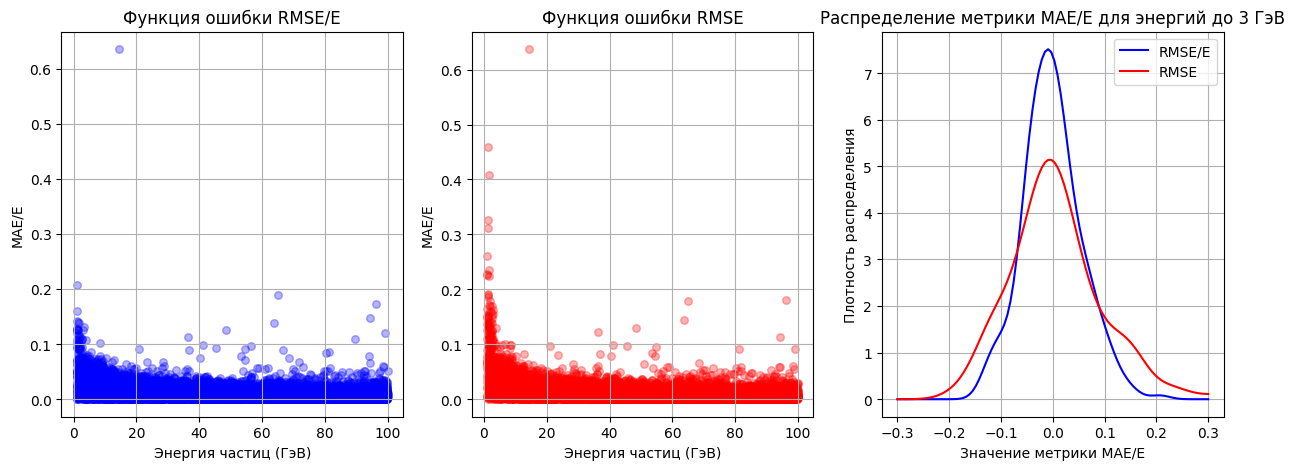
\includegraphics[width=1.0\textwidth]{graphics/exp2_distr_comp.png}
    \caption{}
    \label{graph:loss_distr}
\end{figure}

\section{Обсуждение}

\section{Заключение}

\section{Благодарности}

\newpage 
\printbibliography[heading=bibintoc] 

% \begin{thebibliography}{0}
% 	\bibitem{chirkova18}\hypertarget{chirkova18}{}
% 	\href{https://arxiv.org/abs/1810.10927}
% 	{Nadezhda Chirkova, Ekaterina Lobacheva, Dmitry Vetrov. Bayesian Compression for Natural Language Processing. In EMNLP 2018.}
% \end{thebibliography}

\newpage
\appendix

\section{Пример секции аппендикса}

\end{document}
